\documentclass{standalone}

%----------------------------------------------------------------------------------------------%
%                                 Packages and basic declarations
%----------------------------------------------------------------------------------------------%

\usepackage{amsmath}
\usepackage{mathrsfs}
\usepackage{pgf}
\usepackage{tikz}
\usepackage{verbatim}


\usetikzlibrary{arrows}


\tikzset{
  font={\fontsize{36pt}{32}\selectfont}}

%----------------------------------------------------------------------------------------------%
%----------------------------------------------------------------------------------------------%
%                                            DOCUMENT STARTS
%----------------------------------------------------------------------------------------------%
%----------------------------------------------------------------------------------------------%

\begin{document}

%----------------------------------------------------------------------------------------------%
%                Single RVE with applied constant strain, only debonded
%----------------------------------------------------------------------------------------------%

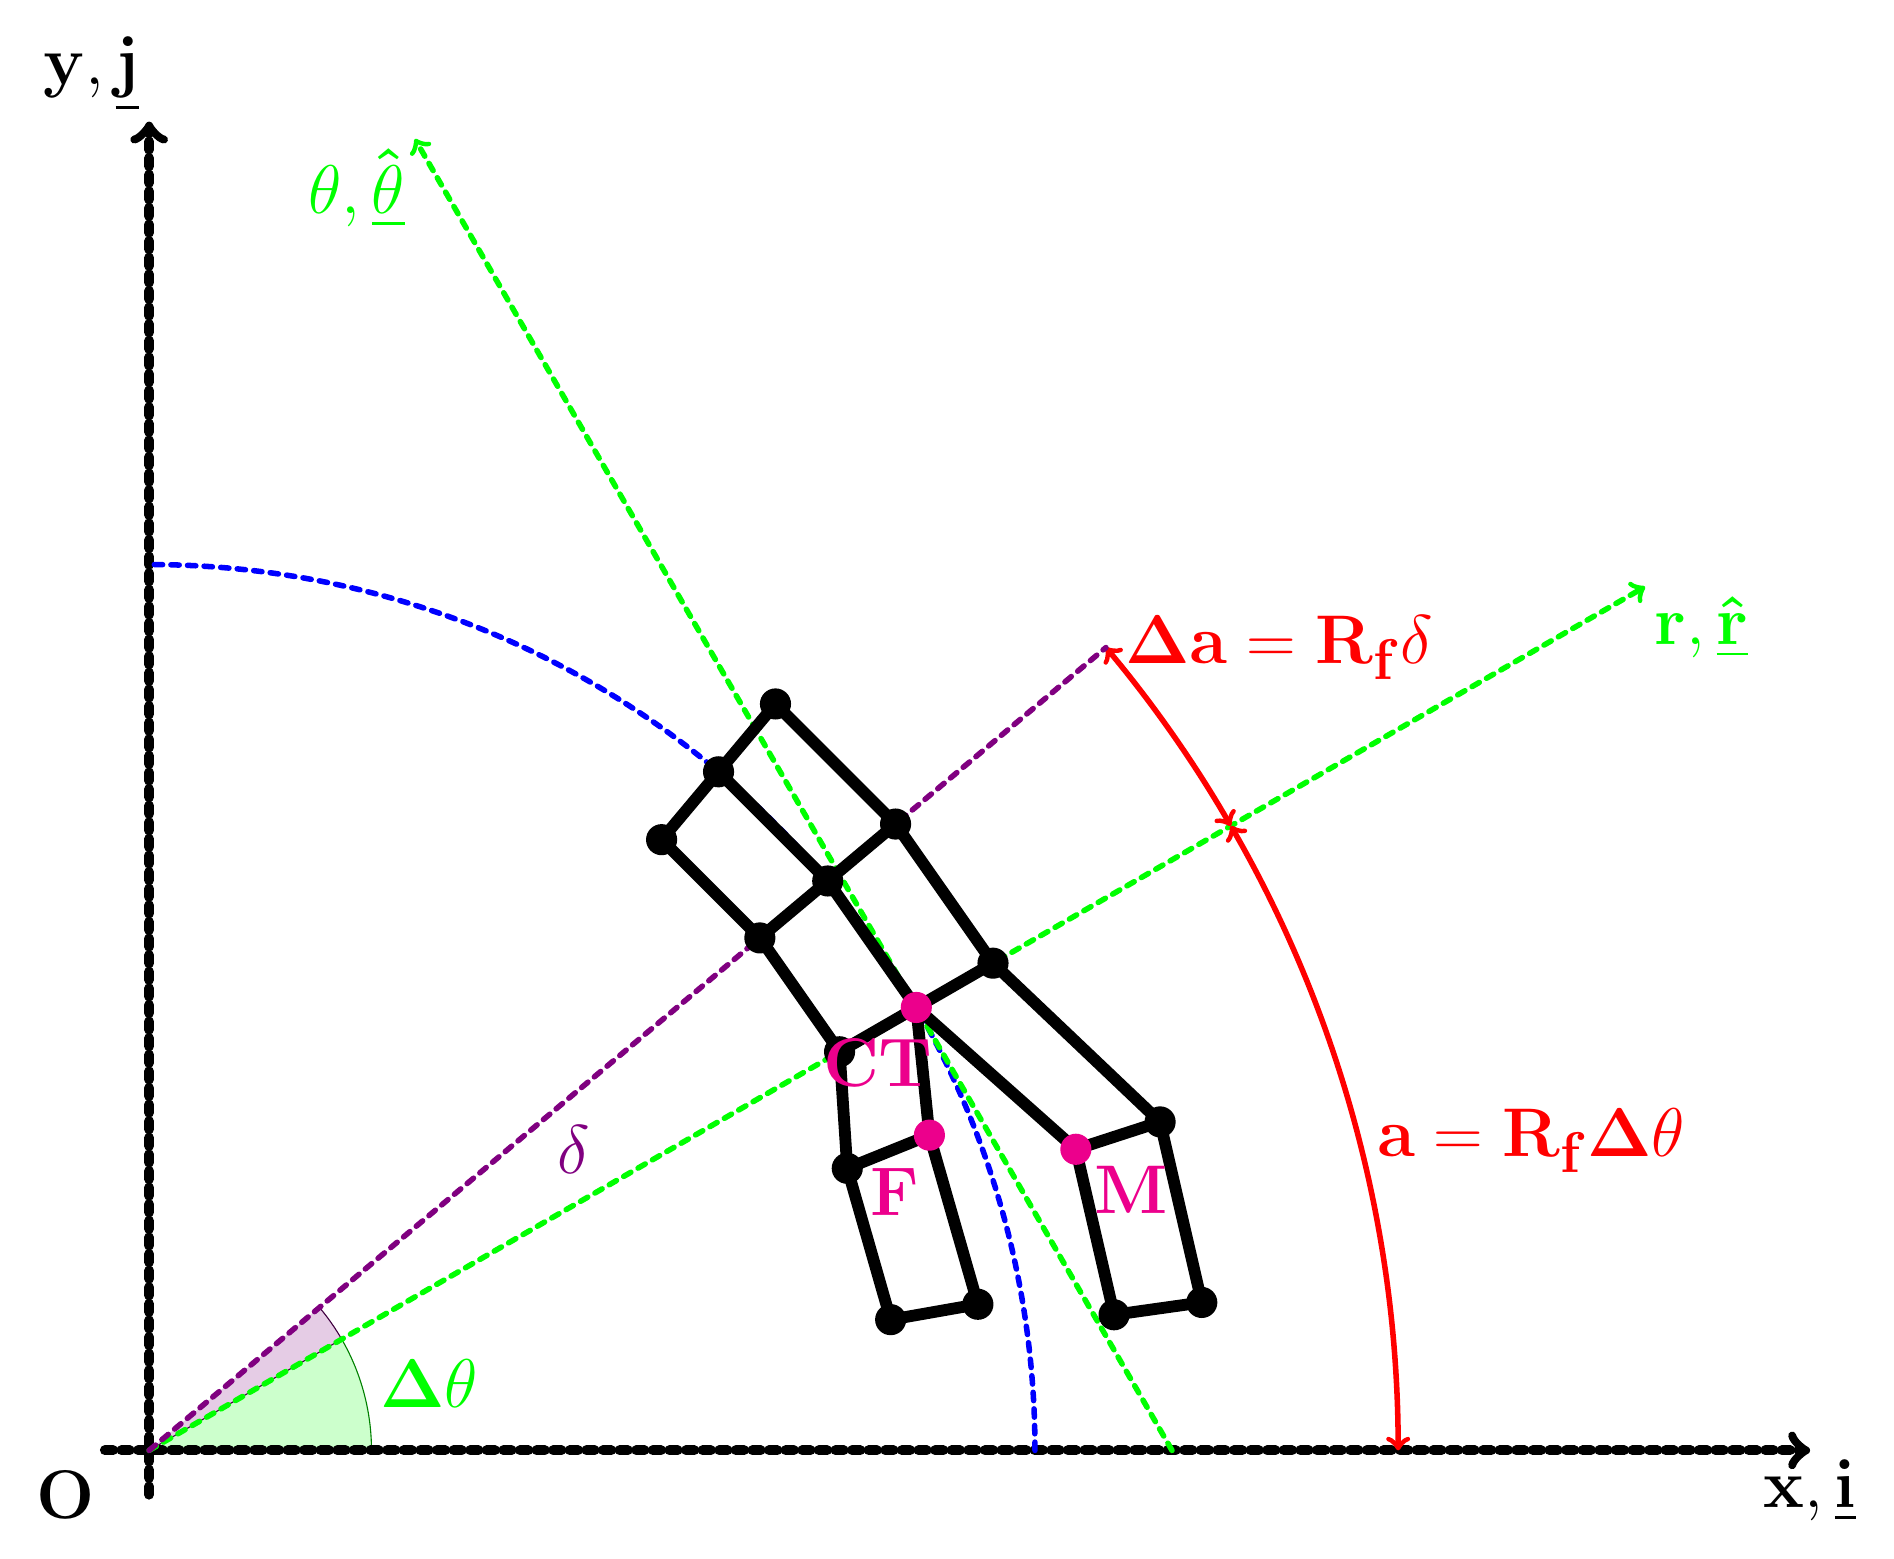
\begin{tikzpicture}[scale=7.5,cap=round,x=1.5cm,y=1.5cm]

%----------------------------------------------------------------------------------------------%
%                                                   CONSTANTS
%----------------------------------------------------------------------------------------------%

\def\pivalue{3.141592653589793238462643383279502884197169399375105820974944592307816406286}

\def\R{1}
\def\lim{1.5}
\def\xC{0.0}
\def\yC{0.0}

\pgfmathsetmacro\xCT{\R*cos(30)}
\pgfmathsetmacro\yCT{\R*sin(30)}
\pgfmathsetmacro\xA{\R*cos(40)}
\pgfmathsetmacro\yA{\R*sin(40)}
\pgfmathsetmacro\xB{\R*cos(50)}
\pgfmathsetmacro\yB{\R*sin(50)}
\pgfmathsetmacro\xC{0.95*\R*cos(22)}
\pgfmathsetmacro\yC{0.95*\R*sin(22)}
\pgfmathsetmacro\xD{0.95*\R*cos(10)}
\pgfmathsetmacro\yD{0.95*\R*sin(10)}
\pgfmathsetmacro\xE{1.10*\R*cos(18)}
\pgfmathsetmacro\yE{1.10*\R*sin(18)}
\pgfmathsetmacro\xF{1.10*\R*cos(8)}
\pgfmathsetmacro\yF{1.10*\R*sin(8)}

\pgfmathsetmacro\xCTBF{0.9*\R*cos(30)}
\pgfmathsetmacro\yCTBF{0.9*\R*sin(30)}
\pgfmathsetmacro\xABF{0.9*\R*cos(40)}
\pgfmathsetmacro\yABF{0.9*\R*sin(40)}
\pgfmathsetmacro\xBBF{0.9*\R*cos(50)}
\pgfmathsetmacro\yBBF{0.9*\R*sin(50)}
\pgfmathsetmacro\xCBF{0.85*\R*cos(22)}
\pgfmathsetmacro\yCBF{0.85*\R*sin(22)}
\pgfmathsetmacro\xDBF{0.85*\R*cos(10)}
\pgfmathsetmacro\yDBF{0.85*\R*sin(10)}

\pgfmathsetmacro\xCTBM{1.1*\R*cos(30)}
\pgfmathsetmacro\yCTBM{1.1*\R*sin(30)}
\pgfmathsetmacro\xABM{1.1*\R*cos(40)}
\pgfmathsetmacro\yABM{1.1*\R*sin(40)}
\pgfmathsetmacro\xBBM{1.1*\R*cos(50)}
\pgfmathsetmacro\yBBM{1.1*\R*sin(50)}
\pgfmathsetmacro\xEBM{1.20*\R*cos(18)}
\pgfmathsetmacro\yEBM{1.20*\R*sin(18)}
\pgfmathsetmacro\xFBM{1.20*\R*cos(8)}
\pgfmathsetmacro\yFBM{1.20*\R*sin(8)}

\pgfmathsetmacro\xG{1.4\R*cos(30)}
\pgfmathsetmacro\yG{1.4\R*sin(30)}

\pgfmathsetmacro\xH{1.4\R*cos(40)}
\pgfmathsetmacro\yH{1.4\R*sin(40)}

\pgfmathsetmacro\xI{0.25\R*cos(30)}
\pgfmathsetmacro\yI{0.25\R*sin(30)}


\def\xFin{0.3}
\pgfmathsetmacro\yFin{-sqrt(3)*\xFin+(\yCT+sqrt(3)*\xCT)}
\pgfmathsetmacro\xIntersect{(\yCT+sqrt(3)*\xCT)/sqrt(3)}

\filldraw[fill=green!20,draw=green!50!black] (0,0) -- (0.25\R,0) arc(0:30:0.25\R);
\filldraw[fill=violet!20,draw=violet!50!black] (0,0) -- (\xI,\yI) arc(30:40:0.25\R);

\draw[->,dashed, line width = 1.25mm] (-0.05,0.0) -- (1.25*\lim,0.0);
\node[anchor=north] at (1.25*\lim,0.0) {\Huge $\mathbf{x,\underline{i}}$};
\draw[->,dashed, line width = 1.25mm] (0.0,-0.05)  -- (0.0,\lim) ;
\node[anchor=south east] at (0.0,\lim) {\Huge $\mathbf{y,\underline{j}}$};

\node[text=black,anchor=east] at (-0.05,-0.05) {\Huge $\mathbf{O}$};

\draw[draw=blue,dashed,line width=2pt](1,0) arc(0:90:\R);
\draw[->,draw=green,dashed,line width=2pt] (0,0)  -- (1.95*\xCT,1.95*\yCT) ;
\draw[->,draw=green,dashed,line width=2pt] (\xIntersect,0)  -- (\xFin,\yFin) ;

\draw[<->,draw=red,line width=2pt](1.4\R,0) arc(0:30:1.4\R);
\draw[<->,draw=red,line width=2pt](\xG,\yG) arc(30:40:1.4\R);

\draw[draw=violet,dashed,line width=2pt] (0,0)  -- (\xH,\yH) ;


\draw[line width=1.5mm] (\xB,\yB) -- (\xA,\yA) -- (\xCT,\yCT)  -- (\xC,\yC)  -- (\xD,\yD) ;
\draw[line width=1.5mm] (\xCT,\yCT)  -- (\xE,\yE)  -- (\xF,\yF) ;
\draw[line width=1.5mm] (\xBBF,\yBBF) -- (\xABF,\yABF) -- (\xCTBF,\yCTBF)  -- (\xCBF,\yCBF)  -- (\xDBF,\yDBF) ;
\draw[line width=1.5mm] (\xBBM,\yBBM) -- (\xABM,\yABM) -- (\xCTBM,\yCTBM)  -- (\xEBM,\yEBM)  -- (\xFBM,\yFBM) ;
\draw[line width=1.5mm] (\xBBM,\yBBM) -- (\xB,\yB) -- (\xBBF,\yBBF) ;
\draw[line width=1.5mm] (\xABM,\yABM) -- (\xA,\yA) -- (\xABF,\yABF) ;
\draw[line width=1.5mm] (\xCTBM,\yCTBM) -- (\xCT,\yCT) -- (\xCTBF,\yCTBF) ;
\draw[line width=1.5mm] (\xDBF,\yDBF) -- (\xD,\yD);
\draw[line width=1.5mm] (\xCBF,\yCBF) -- (\xC,\yC);
\draw[line width=1.5mm] (\xEBM,\yEBM) -- (\xE,\yE);
\draw[line width=1.5mm] (\xFBM,\yFBM) -- (\xF,\yF);

\foreach \Point in {(\xB,\yB),(\xA,\yA),(\xD,\yD),(\xF,\yF)}{
    \fill \Point  circle[radius=0.75pt];
}
\foreach \Point in {(\xBBF,\yBBF),(\xABF,\yABF),(\xCTBF,\yCTBF),(\xCBF,\yCBF),(\xDBF,\yDBF)}{
    \fill \Point  circle[radius=0.75pt];
}
\foreach \Point in {(\xBBM,\yBBM),(\xABM,\yABM),(\xCTBM,\yCTBM),(\xEBM,\yEBM),(\xFBM,\yFBM)}{
    \fill \Point  circle[radius=0.75pt];
}

\fill[fill=magenta] (\xCT,\yCT)  circle[radius=0.75pt];
\fill[fill=magenta] (\xC,\yC)  circle[radius=0.75pt];
\fill[fill=magenta] (\xE,\yE)  circle[radius=0.75pt];

\node[anchor= west,text=green] at (0.25,0.075) {\Huge $\mathbf{\Delta\theta}$};
\node[anchor= west,text=violet] at (0.45,0.34) {\Huge $\mathbf{\delta}$};
\node[anchor= west,text=red] at (1.375\R,0.35) {\Huge $\mathbf{a = R_{f}\Delta\theta}$};
\node[anchor= west,text=red] at (1.01*\xH,\yH) {\Huge $\mathbf{\Delta a = R_{f}\delta}$};
\node[anchor= north west,text=green] at (1.95*\xCT,1.95*\yCT)  {\Huge $\mathbf{r,\hat{\underline{r}}}$};
\node[anchor= north east,text=green] at (\xFin,\yFin)  {\Huge $\mathbf{\theta,\hat{\underline{\theta}}}$};
\node[anchor= north,text=magenta] at (0.95*\xCT,0.95*\yCT)  {\Huge \bf{CT}};
\node[anchor= north east,text=magenta] at (\xC,0.925*\yC)  {\Huge \bf{F}};
\node[anchor= north west,text=magenta] at (1.01*\xE,0.975*\yE)  {\Huge \bf{M}};

%\draw[line width=1.5mm] (4,0) -- (4,-1) -- (2,-1) -- (0,-1) -- (-1.5,-1.25) --  (-1.5,-0.25) -- (0,0);
%\draw[line width=1.5mm] (4,1) -- (4,-1);
%\draw[line width=1.5mm] (2,1) -- (2,-1);
%\draw[line width=1.5mm] (0,1) -- (0,-1);
%\draw[line width=1.5mm] (-2,1.5) -- (-4,1.5) -- (-6,1.5) -- (-6,0.5) -- (-4,0.5) -- (-2,0.5);
%\draw[line width=1.5mm] (-1.5,-1.25) -- (-3.5,-1.25) -- (-5.5,-1.25) -- (-5.5,-0.25) -- (-3.5,-0.25) -- (-1.5,-0.25);
%\draw[line width=1.5mm] (-4,1.5) -- (-4,0.5);
%\draw[line width=1.5mm] (-3.5,-1.25) -- (-3.5,-0.25);
%
%\draw[<->,line width=1.3mm,draw=red] (0,1.75) -- (-2,1.75);
%\node[anchor= south,text=red] at (-1,1.75) {\Huge $\mathbf{\Delta a}$};
%\draw[->,line width=1.3mm,draw=red] (-6,1.75) -- (-2,1.75);
%\node[anchor= south,text=red] at (-4,1.75) {\Huge $\mathbf{a}$};
%\draw[<->,line width=1.3mm,draw=red] (0,1.75) -- (2,1.75);
%\node[anchor= south,text=red] at (1,1.75) {\Huge $\mathbf{\Delta a}$};
%\node[anchor= north,text=red] at (1,1.7) {\Huge \bf{crack closed}};
%\draw[<->,line width=1.3mm,draw=red] (2,1.75) -- (4,1.75);
%\node[anchor= south,text=red] at (3,1.75) {\Huge $\mathbf{\Delta a}$};
%\node[anchor= north,text=red] at (3,1.7) {\Huge \bf{crack closed}};
%
%\draw[dashed,line width=1.5mm,draw=green] (-1.5,-0.25) -- (-1.5,-1.75);
%\draw[dashed,line width=1.5mm,draw=green] (-2,0.5) -- (-2,-1.75);
%\draw[<->,line width=1.5mm,draw=green] (-2,-1.75) -- (-1.5,-1.75);
%\node[anchor= north,text=green] at (-1.75,-1.8) {\Huge $\mathbf{\Delta u_{C}}$};
%
%
%\draw[dashed,line width=1.5mm,draw=green] (-1.5,-0.25) -- (-1,-0.25);
%\draw[dashed,line width=1.5mm,draw=green] (-2,0.5) -- (-1,0.5);
%\draw[<->,line width=1.5mm,draw=green] (-1,-0.25) -- (-1,0.5);
%\node[anchor= west,text=green] at (-1,-0.25+0.375) {\Huge $\mathbf{\Delta w_{C}}$};
%
%\draw[->,line width=1.75mm,draw=blue] (0,0) -- (0,0.5);
%\node[anchor=south east,text=blue] at (0,0.5) {\Huge $\mathbf{Z_{C}^{u}}$};
%\draw[->,line width=1.75mm,draw=blue] (0,0) -- (0,-0.5);
%\node[anchor=north west,text=blue] at (0,-0.5) {\Huge $\mathbf{Z_{C}^{l}}$};
%\draw[->,line width=1.75mm,draw=blue] (0,0) -- (0.5,0);
%\node[anchor= south west,text=blue] at (0.5,0) {\Huge $\mathbf{X_{C}^{l}}$};
%\draw[->,line width=1.75mm,draw=blue] (0,0) -- (-0.5,0);
%\node[anchor= north east,text=blue] at (-0.5,0) {\Huge $\mathbf{X_{C}^{u}}$};
%
%\foreach \Point in {(4,0) , (4,1) , (2,1) , (0,1) , (-2,1.5) , (-2,0.5) , (0,0) , (2,0),(4,-1) , (2,-1) , (0,-1) , (-1.5,-1.25) ,  (-1.5,-0.25),(-2,1.5) , (-4,1.5) , (-6,1.5) , (-6,0.5) , (-4,0.5) , (-2,0.5),(-1.5,-1.25) , (-3.5,-1.25) , (-5.5,-1.25) , (-5.5,-0.25) , (-3.5,-0.25) , (-1.5,-0.25)}{
%    \fill \Point  circle[radius=2pt];
%}
%
%\node[anchor= south,text=red] at (-1,2.5) {};
%\node[anchor= north,text=red] at (-1.75,-2.5) {};
%\node[anchor= east,text=red] at (-7.25,0) {};
%\node[anchor= west,text=red] at (4.75,0) {};


\end{tikzpicture}

\end{document}
